%++++++++++++++++++++++++++++++++++++++++
% Don't modify this section unless you know what you're doing!
\documentclass[letterpaper,14pt]{article}
% \documentclass[letterpaper,17pt]{extreport}
% 8pt, 9pt, 10pt, 11pt, 12pt, 14pt, 17pt, 20pt.
% \usepackage[T1]{fontenc}
% \usepackage{tgbonum}

\usepackage{natbib}
\bibliographystyle{unsrtnat}
\usepackage{tabularx} % extra features for tabular environment
\usepackage{amsmath}  % improve math presentation
\usepackage{graphicx} % takes care of graphic including machinery
\usepackage[margin=1in,letterpaper]{geometry} % decreases margins
%\usepackage{cite} % takes care of citations
\usepackage[final]{hyperref} % adds hyper links inside the generated pdf file
\hypersetup{
	colorlinks=true,       % false: boxed links; true: colored links
	linkcolor=blue,        % color of internal links
	citecolor=blue,        % color of links to bibliography
	filecolor=magenta,     % color of file links
	urlcolor=blue         
}

% additional package
\usepackage{bm}
\usepackage{amssymb}
\usepackage{color}
\usepackage{algorithm}
\usepackage{algorithmic}
\usepackage{amsthm,nccmath}
\usepackage{listings}
\usepackage[numbered,framed]{matlab-prettifier}
% \usepackage{typedref}
\newtheorem{theorem}{Theorem}
\newtheorem{definition}{Definition}
\newtheorem{notation}{Notation}
\newtheorem{corollary}{Corollary}
\newtheorem{lemma}{Lemma}
% \newtheorem{lemma}[theorem]{Lemma}{Lemmas}

% Define a custom color
\definecolor{backcolour}{rgb}{0.95,0.95,0.92}
\definecolor{codegreen}{rgb}{0,0.6,0}

\let\ph\mlplaceholder % shorter macro
\lstMakeShortInline"

\lstset{
  style              = Matlab-editor,
  basicstyle         = \mlttfamily\ttfamily\footnotesize,
  escapechar         = ",
  mlshowsectionrules = true,
	breakatwhitespace	 = false,
	breaklines				 = true,
	keepspaces				 = true,
	numbers						 = left,
	numbersep					 = 5pt,
	showspaces				 = false,
	showstringspaces	 = false,
	showtabs					 = false,              
	tabsize						 = 2,
	backgroundcolor	   = \color{backcolour},
	commentstyle	     = \color{codegreen},
}

%++++++++++++++++++++++++++++++++++++++++

% \makeatletter
% {\LARGE \@title}{\fontsize{40pt}{49.2pt}\selectfont\@title}{}{}
% \makeatother
\begin{document}

\title{APPLIED NUMERICAL METHODS\\Homework \# 1}
\author{Yuhe Guo\quad Student ID: ~}
\date{2021.11.01}
\maketitle

% \input{}
\section*{Question 1}
\textcolor{blue}{[Range, Linear Mapping and Matrix]}
Let $f_1, ..., f_8$ be a set of functions defined on the interval $[1, 8]$ 
with the property that for any numbers $d_1, ..., d_8$, 
there exists a set of  coefficients $c_1, ..., c_8$ such that
 \begin{equation*}
     \sum_{j=1}^8 c_jf_j(i) = d_i,\quad i=1, ..., 8
 \end{equation*}
(a) Show by appealing to the theorems of this lecture 
that $d_1, ..., d_8$ determine $c_1, ..., c_8$ uniquely.
\\
(b)  Let $A$ be the $8 \times 8$ matrix representing the linear mapping 
from data $d_1, ..., d_8$ to coefficients $c_1, ..., c_8$.
What is the $i$, $j$ entry of $A^{-1}$ ?


\subsection*{Answer}
% \subsection*{Proof}
(a). 
For proof, we will use two theorems from APPLIED NUMERICAL
ANALYSIS below:
\begin{theorem}
\label{theorem:range}
Range($A$) is the space spanned by the columns of $A$.
\end{theorem}

\begin{theorem}
\label{theorem:fullrank}
A matrix $A \in \mathbb{C}^{m \times n}$ has full rank 
if and only if maps no two distinct vectors to the same vector.
\end{theorem}

\begin{proof}
    Denote $F = \begin{bmatrix}
        f_1(1) & ... & f_8(1)\\
        ...   & ... & ... \\
        f_1(8) & ... & f_8(8)\\
    \end{bmatrix}$.
    We can re-write the mapping $f$ on $c_1, ..., c_8$ to 
    $d_1, ..., d_8$ in a matrix-vector-product way:
    \begin{equation*}
        \label{eq:q1}
        F
        \begin{bmatrix}
            c_1 \\ ... \\ c_8 \\
        \end{bmatrix} 
        = 
        \begin{bmatrix}
            d_1 \\ ... \\ d_8 
        \end{bmatrix} .
    \end{equation*}

    Note that the value of $d_i$ can be any number, 
    and we can view $[d_i]_{i\in[1,8]}$ to be spanned by
    the columns of $F$, so $Range(F) = 8$. By applying 
    Theorem \ref{theorem:range}, we get that $F$ is full-rank.
    
    So, $d_1, ..., d_8$ determine $c_1, ..., c_8$ uniquely.
    Otherwise, we'll find two different vectors that map 
    the columns of full-rank matrix $F$ to a same vector, 
    which conflicts Theorem \ref{theorem:fullrank}. 
    Until now We have finished sub-question (a).
\end{proof}

(b). As $F$ is full-rank, \eqref{eq:q1} can be written as:
\begin{equation*}
    \label{eq:q1}
    \begin{bmatrix}
        c_1 \\ ... \\ c_8 \\
    \end{bmatrix} 
    = 
    F^{-1}
    \begin{bmatrix}
        d_1 \\ ... \\ d_8 
    \end{bmatrix} .
\end{equation*}

So $A = F^{-1} \rightarrow A^{-1} = F 
\rightarrow A^{-1}_{i,j} = F_{ij} = f_j(i)$.
Until now We have finished sub-question (b).





\section*{Question 2}
\textcolor{blue}{[Rank-one perturbation of the identity]}
2.6. If $u$ and $v$ are m-vectors, 
the matrix $A = I + uv*$ is known as a rank-one perturbation of the identity. 
\begin{itemize}
    \item Show that if $A$ is nonsingular, then its inverse has the form $A^{-1} = I + auv*$ for some scalar $a$, and give an expression for $a$.
    \item For what $u$ and $v$ is $A$ singular? If it is singular, what is $null (A)$?
\end{itemize}



\subsection*{The first part of proof}
Suppose that $A$ is non-singular, 
let $B = I + auv^*$, we will prove that for any $A$,
we can find a corresponding $a$, and thus a corresponding $B$,
so that $B = A^{-1}$.

If $AB = I$, we get:
\begin{align*}
    AB = I &\rightarrow (I + uv^*)(I + auv^*) = I\\
           &\rightarrow I + auv^* + uv^* + au(v^*u)v* = I \\
           &\rightarrow (a + 1 + av^*u)uv^* = 0 \\
           &\rightarrow a(1 + v^*u) + 1 = 0 \ or\ uv^* = 0
\end{align*}

% which indicates that $uv^* = 0$ or $(a + 1 +v^*u)=0$. 
As been given,  $rank(u) = rank(v) = 1 > 0$,
so the $a$ we need satisfies:
\begin{equation}
    \label{eq:1.1}
    a(1 + v^*u) = -1
\end{equation}

Next we show that $v^*u \neq -1$. Assume that $v^*u = -1$, then 
$Au = (I + uv^*)u = u + u*(-1) =  \mathbf{0}, $ conflicting that
$u\neq \mathbf{0}$ and $A$ is non-singular.

So from \eqref{eq:1.1} we further get:
\begin{equation}
a = - \dfrac{1}{1+v^*u}
\end{equation}

\subsection*{The second part of proof}

In this part, we show that $v^*u = -1$ is the necessary and sufficient condition
when $A$ is singular.

\subsubsection*{sufficiency}
As been shown in the former part,
when $v^*u = -1$,
$Au = (I + uv^*)u = u + u*(-1) =  \mathbf{0}$,
then $A$ is singular.

\subsubsection*{necessity}
Once $v^*u \neq -1$, according to the former part,
we can construct a matrix $ B = I - \dfrac{1}{1+ v^*u}uv^*$
that $AB = I$, which indicates that $A$ is non-singular.
So we have proved the necessity.

\subsubsection*{The Null Space of A}
\begin{align*}
    Ax &= 0 \\
    \rightarrow (I + uv^*)x &= 0 \\
    \rightarrow x &= - (v^*x)u \\
    \rightarrow x & // u
    \rightarrow Null(A) = span([u])
\end{align*}






\section*{Question 3}
\textcolor{blue}{[Singular Values of Rotated Matrix]} Suppose $A$ is an $m \times n$ matrix and $B$ is the $n \times m$ matrix obtained by
rotating $A$ ninety degrees clockwise on paper (not exactly a standard mathematical transformation!). 
Do $A$ and $B$ have the same singular values? 
Prove that the answer is yes or give a counterexample.

\subsection*{Answer}
Yes. 

\subsection*{Proof}
\begin{notation}
We use $A^{R}$ as a  notation for the  ninety-degree clock-wisely rotated $A$,
and $A^T$ for the transpose of $A$.
\end{notation}

For proof, we will use the theorem and corollary below:
\begin{theorem}
\label{theorem:singular}
The nonzero singular values of A are the square roots of the nonzero eigenvalues of $A*A$ or $AA*$.[NLA Theorem 5.4]
\end{theorem}

We will also use the immediate corollary of \ref{theorem:singular} below:
\begin{corollary}
\label{corollary:singular}
For any matrix  $M \in \mathbb{R}^{m \times n}$,
$AA^*$ and $A^*A$ share the same singular values.
\end{corollary}

\begin{lemma}[Relation between $A^{R}$ and $A^T$]
\label{lem:lem1}
For any matrix $A \in \mathbb{R}^{m \times n}$,
% $A^T, A^R \in \mathbb{R}^{n \times m}$,
$A^T_{i,j}=A^R_{i,m-j-1}$ 
\end{lemma}

\begin{proof}
$A^T_{i,j} = A{j,i} = A^R_{i,m-j-1}$.
\end{proof}

\begin{lemma}[Singular value of $A^{R}$ and $A^T$]
\label{lem:lem2}
$A^{R}$ and $A^T$ share the same singular values.
\end{lemma}

\begin{proof}
Denote $A^T$ to be $C$,  $A^R$ to be $D$.
According to \ref{lem:lem1},
the elements in each row $i$ of $C$ and $D$ are the same,
they are just permuted (more precisely, permuted in reversed orders), and the permutation are parallel among each row. So the inner product of any two rows in $C$ and $D$ are the same:
\begin{equation*}
    \langle C[i,:], C[j,:] \rangle = \langle D[i,:], D[j,:] \rangle
\end{equation*}

So: 
\begin{equation}
    \label{eq:cct}
    CC^T = [\langle C[i,:], C[j,:] \rangle]_{ij} = 
    \langle D[i,:], D[j,:] \rangle = DD^T
\end{equation}

By Theorem \ref{theorem:singular} and \eqref{eq:cct} we derive that $C$ and $D$ share the same singular values . Thus, we have finished the proof of Lemma \ref{lem:lem2}.
\end{proof}

\begin{proof}
Back to the question. By \ref{lem:lem2}, $B$ shares the same singular values with $A^T$; By \ref{corollary:singular}, $A^T$ shares the same singular values with $A$. So  $A$ and $B$ have the same singular values.
\end{proof}




\section*{Question 4}
\textcolor{blue}{[Practice with SVD]}


Consider the matrix
\begin{align*}
A = \begin{bmatrix}
-2 & 11\\
-10 & 5\\
\end{bmatrix}    
\end{align*}


\begin{enumerate}
    \item Determine, on paper, a real SVD of $A$ in the form $A = U \Sigma V^T$. The SVD is not unique, so find the one that has the minimal number of minus signs in $U$ and $V$;
    \item List the singular values, left singular vectors, and right singular vectors of $A$. 
    Draw a careful, labeled picture of the unit ball in $\mathbb{R}^2$ and its image under $A$, 
    together with the singular vectors, 
    with the coordinates of their vertices marked;
    \item What are the 1-, 2-, $\infty$-, and Frobenius norms of $A$?
    \item Find $A^{-1}$ not directly, but via the SVD;
    \item Find the eigenvalues $\lambda_1$,  $\lambda_2$ of $A$;
    \item Verify that det $A$ = $\lambda_1\lambda_2$ and $|\det A|=\sigma_1\sigma_2$;
    \item What is the area of the ellipsoid onto which $A$ maps the unit ball in $\mathbb{R}^2$?
\end{enumerate}



\subsection*{Answer}
\subsubsection*{1. SVD Calculation}
\begin{align*}
A &= U \Sigma V^T = \begin{bmatrix}
-2 & 11\\
-10 & 5\\
\end{bmatrix} \\  
\xrightarrow{} 
AA^T &= U \Sigma^2 U^T = \begin{bmatrix}
125 & 75\\
75 & 125
\end{bmatrix} ,\\
A^TA &= V \Sigma^2 V^T = \begin{bmatrix}
    104 & -72\\
    -72 & 146
    \end{bmatrix}
% \xrightarrow{} 
\end{align*}

Conduct eigen decomposition on $AA^T$ and $A^TA$, we get:
\begin{equation*}
    U  = 
    \begin{bmatrix}
        -\sqrt{2}/2 & \sqrt{2}/2\\
        \sqrt{2}/2 & \sqrt{2}/2\\
    \end{bmatrix}, \quad
    \Sigma = 
    \begin{bmatrix}
        5\sqrt{2} & 0\\
        0 & 10\sqrt{2}\\
    \end{bmatrix}, \quad
    V = 
    \begin{bmatrix}
        -4/5 & -3/5\\
        -3/5 & 4/5 
    \end{bmatrix}
\end{equation*}

We adjust $U$ and $V$ so that we get
the minimal number of minus signs,
we turn the sign of $U$'s first column and 
$V$'s first column, and get:

\begin{equation}
    \label{eq:SVD}
    U  = 
    \begin{bmatrix}
        \sqrt{2}/2 & -\sqrt{2}/2\\
        \sqrt{2}/2 & \sqrt{2}/2\\
    \end{bmatrix}, \quad
    \Sigma = 
    \begin{bmatrix}
        5\sqrt{2} & 0\\
        0 & 10\sqrt{2}\\
    \end{bmatrix}, \quad
    V = 
    \begin{bmatrix}
        4/5 & 3/5\\
        -3/5 & 4/5 
    \end{bmatrix}
\end{equation}




\subsubsection*{2. Visualization of SVD.}
From \eqref{eq:SVD} we directly get:
% Singular values: $5\sqrt{2},10\sqrt{2}$; \\
\begin{itemize}
    \item Singular values:
    \begin{equation}
        \label{eq:sigma}
        \sigma_1 = 5\sqrt{2},\quad \sigma_2 = 10\sqrt{2};
    \end{equation}
    \item Left singular vectors:  $[-\sqrt{2}/2, \sqrt{2}/2]^T, [\sqrt{2}/2, \sqrt{2}/2]^T$ ;
    \item Right singular vectors : $[4/5, -3/5]^T, [3/5, 4/5]^T$.
\end{itemize}

% Left singular vectors: $[-\sqrt{2}/2, \sqrt{2}/2]^T, [\sqrt{2}/2, \sqrt{2}/2]^T$ \\
% Right singular vectors : $[4/5, -3/5]^T, [3/5, 4/5]^T$.\\
The unit ball's image under $A$ is show as follow:
\begin{figure}[H]
    \centering
    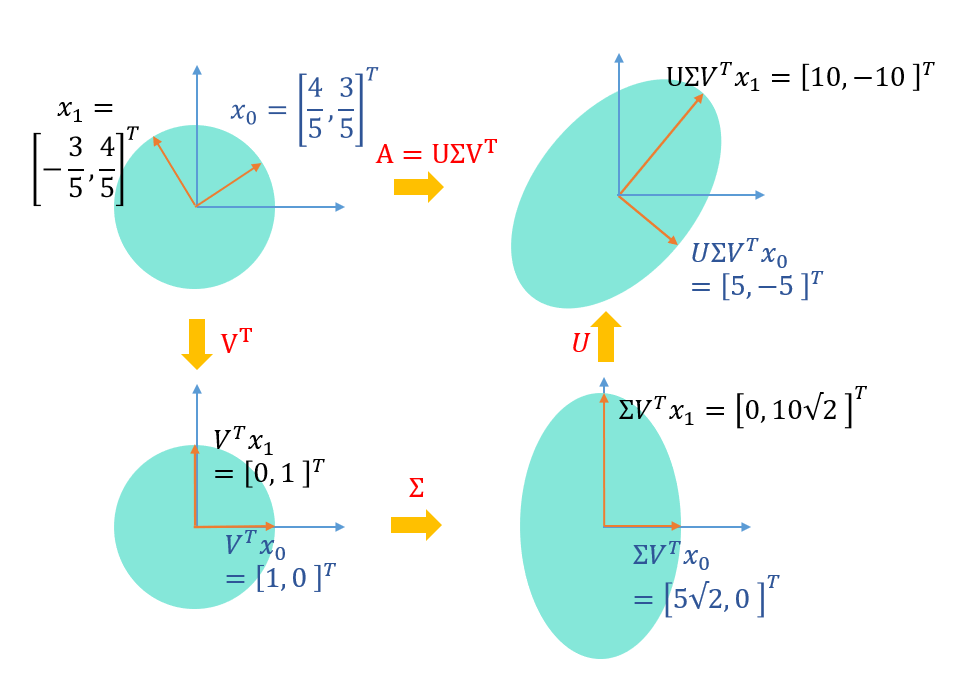
\includegraphics[width=1\textwidth]{SVD_yuhe.png}
    \caption{The unit ball's image under $A$}
    \label{fig:mapping A}
  \end{figure}

\subsubsection*{3. Matrix's Norms}
% 1-, 2-, $\infty$-, and Frobenius norms of $A$
$\|A\|_1 = 28$,\\
$\|A\|_2 = 5\sqrt{10}$,\\
$\|A\|_\infty = 11$,\\
$\|A\|_F = 5\sqrt{10}$

\subsubsection*{4. $A^{-1}$ By SVD \textcolor{red}{[TODO: Check again!]}}
\begin{flalign*}
A^{-1} &= (U \Sigma V^T)^{-1} = {V \Sigma^{-1} U^T} 
    = \begin{bmatrix}
            0.05 & 0.11\\
            -0.1 & -0.02\\
            \end{bmatrix}  &&
\end{flalign*}

\subsubsection*{5. Eigen Values of $A^{-1}$}
The charateristic polynomial of $A$ is:
\begin{equation*}
    p_A(\lambda) = \det(A-\lambda I) = \lambda^2 - 3\lambda + 100,
\end{equation*}
so that we obtain:
%  $\lambda_1 = \dfrac{3+\sqrt{-391}}{2}$ and  $\lambda_2 = \dfrac{3-\sqrt{-391}}{2}$.
\begin{align}
    \label{eq:eigenvalues}
    \left
    \{ \begin{aligned}
        \lambda_1 &= \dfrac{3+\sqrt{-391}}{2} \\ \lambda_2 &= \dfrac{3-\sqrt{-391}}{2}
    \end{aligned}
    \right.
\end{align}

\subsubsection*{6. Relationship of Eigen Values and Matrixs' Determinant and Trace}
From \eqref{eq:eigenvalues} and \eqref{eq:sigma}, we get:
\begin{align*}
    % \label{eq:eigenvalues}
    \left
    \{ \begin{aligned}
        \lambda_1\lambda_2 &= 100 = \det A \\ 
        \sigma_1\sigma_2   &= 100 = |\det A|\\
    \end{aligned}
    \right.
\end{align*}




\subsubsection*{7. Ellipsoid Mapped $A^{-1}$}
Figure \ref{fig:mapping A} has been shown in sub-question 2,
now we describe the mapped-to ellipsoid analytically:
\\
The unit ball before mapped by $A$ is :
\begin{equation*}
    \{\ (x,y) \ |\ [x,y]     
                    \begin{bmatrix}
                        1 & 0\\
                        0 & 1\\
                    \end{bmatrix}
                    \begin{bmatrix}
                        x\\
                        y\\
                    \end{bmatrix}   \leq 1  
    \}.
\end{equation*}
\\
After being mapped by $A$, the set of points comes to:
\begin{equation*}
    \{\ (x,y) \ |\ ([x,y]A^T)
                    \begin{bmatrix}
                        1 & 0\\
                        0 & 1\\
                    \end{bmatrix}
                    (A
                    \begin{bmatrix}
                        x\\
                        y\\
                    \end{bmatrix})  \leq 1  
    \},
\end{equation*}
which can be written as:
\begin{equation}
    \label{eq:analytical_epi}
    \{\ (x,y) \ |\ [x,y]A^TA
                    \begin{bmatrix}
                        x\\
                        y\\
                    \end{bmatrix}  \leq 1  
    \}.
\end{equation}
Equation \eqref{eq:analytical_epi} is just the analytical solution
of obtain ellipsoid.

\section*{Question 5}
\textcolor{blue}{[(Orthogonal) Projector onto Column Range]} Consider the matrices:

\begin{align*}
    A = \begin{bmatrix}
        1 & 0\\ 0 & 1\\ 1 & 0
    \end{bmatrix},\quad
    B = \begin{bmatrix}
        1 & 2\\ 0 & 1\\ 1 & 0
        \end{bmatrix}
    \end{align*}

Answer the following questions by hand calculation.

(a) What is the orthogonal projector $P$ onto $range(A)$,
and what is the image under $P$ of vector $[1,2,3]^*$?

(b) Same question for $B$.

\subsection*{Answer}

(a). The projector is: \begin{equation*}
    P = A(A^TA)^{-1}A^T = 
    \begin{bmatrix}
        \frac{1}{2} & 0 & \frac{1}{2} 
        \\ 0 & 1 & 0
        \\ \frac{1}{2} & 0 & \frac{1}{2}
    \end{bmatrix}.\quad
\end{equation*}

The image under $P$ of $[1,2,3]^*$ is:
\begin{equation*}
    P[1, 2, 3]^* = [2, 2, 2]^*.    
\end{equation*}

(b). The projector is: \begin{equation*}
    P = B(B^TB)^{-1}B^T = 
    \begin{bmatrix}
        5/6 & 1/3 & 1/6 
        \\ 1/3 & 1/3 & -1/3
        \\ 1/6 & -1/3 & 5/6
    \end{bmatrix}.\quad
\end{equation*}

The image under $P$ of $[1,2,3]^*$ is:
\begin{equation*}
    P[1, 2, 3]^* = [2, 0, 2]^*.    
\end{equation*}





\section*{Question 6}
\textcolor{blue}{[QR Factorization]} Consider again the matrices A and B of question 6.


(a)  Using any method you like, determine (on paper) a reduced QR factorization $A = \hat{Q}\hat{R}$ and a full QR factorization $A = QR$.


(b)  Again using any method you like, determine reduced and full QR factorizations $B = \hat{Q}\hat{R}$ and $B = QR$.

% \begin{align*}
    % A = \begin{bmatrix}
    %     1 & 0\\ 0 & 1\\ 1 & 0
    % \end{bmatrix},\quad
%     B = \begin{bmatrix}
%         1 & 2\\ 0 & 1\\ 1 & 0
%         \end{bmatrix}
%     \end{align*}

\subsection*{Answer}

(a1)\textcolor{blue}{[Reduced QR factorization of $A$]}. 
Denote the reduced QR factorization of $A$ as
$A = \hat{Q}\hat{R}$, $
    \hat{Q} \in \mathbb{R}^{3 \times 2},
    \hat{R} \in \mathbb{R}^{2 \times 2} 
    $,

\begin{align*}
    &A = [\mathbf{a_1}, \mathbf{a_2}],
    \quad 
    \hat{Q} = [\mathbf{q_1}, \mathbf{q_2}], \quad
    \hat{R} = \begin{bmatrix}
                r_{11} & r_{12}\\ 0 & r_{22}
            \end{bmatrix},\\
    &\mathbf{a_1, a_2} \in \mathbb{R}^{3\times 1}, \quad
    \mathbf{q_1, q_2} \in \mathbb{R}^{3\times 1},\\
    & r_{11}, r_{12}, r_{22} \in \mathbb{R}.
\end{align*}

As been given, $\mathbf{a_1} \bot \mathbf{a_2}$,
so we directly derive that:
% \begin{equation}
%     \mathbf{q_1} = \mathbf{a_1}/\|\mathbf{a_1}\|, \quad
%     \mathbf{q_2} = \mathbf{a_2}/\|\mathbf{a_2}|
% \end{equation}

\begin{align}
    \label{eq:6.1}
    \mathbf{q_1} &= \mathbf{a_1}/\|\mathbf{a_1}\|, \quad r_{11} = \|\mathbf{a_1}\|\\
    \label{eq:6.2}
    \mathbf{q_2} &= \mathbf{a_2}/\|\mathbf{a_2}\|, \quad r_{22} = \|\mathbf{a_2}\|
\end{align},
and 
\begin{align}
    \mathbf{a_2} &= r_{12}\mathbf{q_1} + r_{22}\mathbf{q_2}
    % \Rightarrow r_{12}\mathbf{q_1} + r_{22}\mathbf{q_2} = \mathbf{a_2}
    \nonumber \\
    \Rightarrow
    \langle\mathbf{a_2}, \mathbf{q_1} \rangle 
    &=  
    r_{12} \langle\mathbf{q_1}, \mathbf{q_1} \rangle 
    + r_{22}\langle\mathbf{q_2}, \mathbf{q_1} \rangle 
    \nonumber \\
    \label{eq:6.3}
    \Rightarrow r_{12} &= 0.
\end{align}

Compounding equations \eqref{eq:6.1} \eqref{eq:6.2} and \eqref{eq:6.3}, 
we get we the reduced QR factorization of $A$:
\begin{align*}
    \hat{Q} = \begin{bmatrix}
        \sqrt{2}/2 & 0\\ 0 & 1\\ \sqrt{2}/2 & 0
    \end{bmatrix},\quad
    \hat{R} = \begin{bmatrix}
        \sqrt{2} & 0\\ 0 & 1
        \end{bmatrix}
    \end{align*}


(a2)\textcolor{blue}{[Full QR factorization of $A$]}. 
Denote the full QR factorization of $A$ as
$A = QR$, $
    Q \in \mathbb{R}^{3 \times 3},
    R \in \mathbb{R}^{3 \times 2} 
    $,
note that in the equations below, 
all the values except for $\mathbf{q_3}$
keep the same with in reduced QR factorization:

\begin{align*}
    A = [\mathbf{a_1}, \mathbf{a_2}],
    \quad 
    Q = [\mathbf{q_1}, \mathbf{q_2},\textcolor{red}{\mathbf{q_3}}], \quad
    R = \begin{bmatrix}
                r_{11} & r_{12} 
                \\ 0 & r_{22} 
                \\ 0 & 0 
            \end{bmatrix},\\
    % \mathbf{a_1, a_2, q_1, q_2} \in \mathbb{R}^{2\times 1},
    % \quad  r_{11}, r_{12}, r_{22} \in \mathbb{R}.
\end{align*}

As $\mathbf{q_3} \bot \mathbf{q_1}$ and 
$\mathbf{q_3} \bot \mathbf{q_2} $, 
$\mathbf{q_3} \in Null(\hat{Q})$,


\begin{align*}
    \hat{Q}^T\mathbf{q_3} &= 0, \quad \|\mathbf{q_3}\| = 1 \nonumber \\
    \Rightarrow&
    \mathbf{q_3} = \pm [\sqrt{2}/2, 0, -\sqrt{2}/2]^T
\end{align*}

Let $\mathbf{q_3} = [\sqrt{2}/2, 0, -\sqrt{2}/2]^T$, we get
the full QR factorization of $A$
:
\begin{align*}
    Q = \begin{bmatrix}
        \sqrt{2}/2 & 0 & \sqrt{2}/2 \\ 0 & 1 & 0\\ \sqrt{2}/2 & 0 & -\sqrt{2}/2\
    \end{bmatrix},\quad
    R = \begin{bmatrix}
        \sqrt{2} & 0\\ 0 & 1 \\ 0 & 0
        \end{bmatrix}
    \end{align*}



(b1)\textcolor{blue}{[Reduced QR factorization of $B$]}. 
Denote the reduced QR factorization of $B$ as
$B = \hat{Q}\hat{R}$, $
    \hat{Q} \in \mathbb{R}^{3 \times 2},
    \hat{R} \in \mathbb{R}^{2 \times 2} 
    $,

\begin{align*}
    &B = [\mathbf{b_1}, \mathbf{b_2}],
    \quad 
    \hat{Q} = [\mathbf{q_1}, \mathbf{q_2}], \quad
    \hat{R} = \begin{bmatrix}
                r_{11} & r_{12}\\ 0 & r_{22}
            \end{bmatrix},\\
    &\mathbf{b_1, b_2}  \in \mathbb{R}^{3\times 1}, 
    \mathbf{q_1, q_2} \in \mathbb{R}^{3\times 1}\\
    &r_{11}, r_{12}, r_{22} \in \mathbb{R}.
\end{align*}

By the inherent property of QR factorization, 

\begin{align*}
    &\mathbf{q_1} \bot \mathbf{q_2},\\
    &span[\mathbf{q_1}] = span[\mathbf{b_1}],\\
    &span[\mathbf{q_1, q_2}] = span[\mathbf{b_1, b_2}]    
\end{align*}
we derive that:

\begin{align}
    \mathbf{q_1} &= \mathbf{b_1}/\|\mathbf{b_1}\|, \quad r_{11} = \|\mathbf{b_1}\|
    \nonumber \\
    \Rightarrow
    \label{eq:6.4} 
    \mathbf{q_1} &= [\sqrt{2}/2, 0, \sqrt{2}/2]^T, \quad r_{11} = \sqrt{2} 
\end{align},

and 
\begin{align}
    \label{eq:6.5}
    \mathbf{b_2} &= r_{12}\mathbf{q_1} + r_{22}\mathbf{q_2}
    \\
    \Rightarrow
    \langle\mathbf{b_2}, \mathbf{q_1} \rangle 
    &=  
    r_{12} \langle\mathbf{q_1}, \mathbf{q_1} \rangle 
    + r_{22}\langle\mathbf{q_2}, \mathbf{q_1} \rangle 
    \nonumber \\
    \label{eq:6.6}
    \Rightarrow r_{12} &= \langle\mathbf{b_2}, \mathbf{q_1} \rangle =  \sqrt{2}.
\end{align}

Feed \eqref{eq:6.6} into \eqref{eq:6.5}, and apply $\|\mathbf{q_2}\| = 1$we get:
\begin{align}
    r_{22}\mathbf{q_2} &= \mathbf{b_2} - r_{12}\mathbf{q_1} = [1, 1, -1]^T
    \nonumber \\
    \label{eq:6.7}
    &\Rightarrow r_{22} = \sqrt{3}, \mathbf{q_2} = [\sqrt{3}/3, \sqrt{3}/3, -\sqrt{3}/3]
\end{align}

Compounding equations \eqref{eq:6.4} to \eqref{eq:6.7}, 
we get we the reduced QR factorization of $B$:
\begin{align*}
    B = \hat{Q}\hat{R}, \quad
    \hat{Q} = \begin{bmatrix}
        \sqrt{2}/2 & \sqrt{3}/3\\ 0 & \sqrt{3}/3\\ \sqrt{2}/2 & -\sqrt{3}/3
    \end{bmatrix},\quad
    \hat{R} = \begin{bmatrix}
        \sqrt{2} & \sqrt{2} \\ 0  & \sqrt{3}
        \end{bmatrix}.
    \end{align*}





(b2)\textcolor{blue}{[Full QR factorization of $B$]}. 
Denote the full QR factorization of $B$ as
$B = QR$, $
    Q \in \mathbb{R}^{3 \times 3},
    R \in \mathbb{R}^{3 \times 2} 
    $,
note that in the equations below, 
all the values except for $\mathbf{q_3}$
keep the same with in reduced QR factorization:

\begin{align*}
    B = [\mathbf{b_1}, \mathbf{b_2}],
    \quad 
    Q = [\mathbf{q_1}, \mathbf{q_2},\textcolor{red}{\mathbf{q_3}}], \quad
    R = \begin{bmatrix}
                r_{11} & r_{12} 
                \\ 0 & r_{22} 
                \\ 0 & 0 
            \end{bmatrix},\\
    % \mathbf{a_1, a_2, q_1, q_2} \in \mathbb{R}^{2\times 1},
    % \quad  r_{11}, r_{12}, r_{22} \in \mathbb{R}.
\end{align*}

As $\mathbf{q_3} \bot \mathbf{q_1}$ and 
$\mathbf{q_3} \bot \mathbf{q_2} $, 
$\mathbf{q_3} \in Null(\hat{Q})$,

\begin{align*}
    \hat{Q}^T\mathbf{q_3} &= 0, \quad \|\mathbf{q_3}\| = 1 \nonumber \\
    \Rightarrow&
    \mathbf{q_3} = \pm [-\sqrt{6}/6, \sqrt{6}/3, \sqrt{6}/6]^T
\end{align*}

Let $\mathbf{q_3} = [-\sqrt{6}/6, \sqrt{6}/3, \sqrt{6}/6]^T$, we get
the full QR factorization of $B$
:
\begin{align*}
    B = QR, \quad
    Q = \begin{bmatrix}
        \sqrt{2}/2 & \sqrt{3}/3 & -\sqrt{6}/6\\ 0 & \sqrt{3}/3 & \sqrt{6}/3\\ \sqrt{2}/2 & -\sqrt{3}/3 & \sqrt{6}/6
    \end{bmatrix},\quad
    R = \begin{bmatrix}
        \sqrt{2} & \sqrt{2}  \\ 0  & \sqrt{3}  \\ 0 & 0
        \end{bmatrix}.
    \end{align*}
 
\section*{Question 7}
\textcolor{blue}{[QR Factorization with MATLAB Householder]} 

(a) Write a Matlab function $[W,R] = house(A)$ that computes an implicit representation of a full QR factorization 
$A = QR$ of an $m \times n$ matrix $A$ with $m > n$ using Householder reflections. 
The output variables are a lower-triangular matrix $W \in \mathbb{C}^{m \times n}$ 
whose columns are the vectors $v_k$ defining the successive Householder reflections, 
and a triangular matrix $R \in \mathbb{C}^{n \times n}$.

(b) Write a Matlab function $Q = formQ(W)$ that takes 
the matrix $W$ produced by $house$ as input 
and generates a corresponding $m \times m$ orthogonal matrix $Q$.

\section*{Question 8}
\textcolor{blue}{[MATLAB]}

11.3. Take m = 50, n = 12. Using Matlab's linspace, define t to be the m-vector corresponding to linearly spaced grid points from 0 to 1. Using Matlab's vander and fliplr, define A to be the m x n matrix associated with least squares fitting on this grid by a polynomial of degree n — 1. Take b to be the function cos(4t) evaluated on the grid. Now, calculate and print (to sixteen-digit precision) the least squares coefficient vector x by six methods: (a) Formation and solution of the normal equations, using Matlab's \, (b) QR factorization computed by mgs (modified Gram-Schmidt, Exercise 8.2), (c) QR factorization computed by house (Householder triangularization, Exercise 10.2),
(d) QR factorization computed by Matlab's qr (also Householder triangu-larization),
(e) x = A\b in Matlab (also based on QR factorization),
(f) SVD, using Matlab's svd.
(g) The calculations above will produce six lists of twelve coefficients. In each list, shade with red pen the digits that appear to be wrong (affected by rounding error). Comment on what differences you observe. Do the normal equations exhibit instability? You do not have to explain your observations.
\section*{Question 9}
\textcolor{blue}{[Hadmad]}

% \input{Q10_Add_2}
% https://math.stackexchange.com/questions/3892626/singular-values-of-product-of-matrices
% \section{LASSO By ADMM}

Given $y \in \mathbb{R}^{n}, X \in \mathbb{R}^{n \times p}$, recall the lasso problem:
$$
\min _{\beta} \frac{1}{2}\|y-X \beta\|_{2}^{2}+\lambda\|\beta\|_{1}
$$


$$
\min _{\beta} \frac{1}{2}\|y-X \beta\|_{2}^{2}+\lambda\|\beta\|_{1}
$$

We can rewrite this as:
$$
\min _{\beta, \alpha} \frac{1}{2}\|y-X \beta\|_{2}^{2}+\lambda\|\alpha\|_{1} \text { subject to } \beta-\alpha=0
$$

\begin{align}
    &\beta^{(k)}=\left(X^{T} X+\rho I\right)^{-1}\left(X^{T} y+\rho\left(\alpha^{(k-1)}-w^{(k-1)}\right)\right) \\
    &\alpha^{(k)}=S_{\lambda / \rho}\left(\beta^{(k)}+w^{(k-1)}\right) \\
    &w^{(k)}=w^{(k-1)}+\beta^{(k)}-\alpha^{(k)}
\end{align}


% \section{[YH]LASSO By ADMM}

Given $x \in \mathbb{R}^{n}, \Psi \in \mathbb{R}^{n \times p}$, recall the lasso problem:
$$
\min _{\alpha} \frac{1}{2}\|x-\Psi \alpha\|_{2}^{2}+\gamma\|\alpha\|_{1}
$$



We can rewrite this as:
$$
\min _{\alpha, y} \frac{1}{2}\|x-\Psi \alpha\|_{2}^{2}+\gamma\|y\|_{1} \text { subject to } \alpha-y=0
$$

\begin{align}
    &\alpha^{(k)}=\left(\Psi^{T} \Psi+\rho I\right)^{-1}\left(\Psi^{T} x+\rho\left(y^{(k-1)}-z^{(k-1)}\right)\right) \\
    &y^{(k)}=S_{\gamma / \rho}\left(\alpha^{(k)}+z^{(k-1)}\right) \\
    &z^{(k)}=z^{(k-1)}+\alpha^{(k)}-y^{(k)}
\end{align}


%++++++++++++++++++++++++++++++++++++++++

% \bibliography{refs}

\end{document}
